% !TEX root = ../Thesis.tex
% !TEX spellcheck = en-US

\chapter{Comparative Analysis}
\label{ch:comparative}

In this chapter, the results of the experimentation with and in-depth study of GNS3, Kathará, and CORE (chapters~\ref{ch:gns3}, \ref{ch:kathara}, and~\ref{ch:core}, respectively) are exposed in a comparative way, so that the strengths and weaknesses of each one---either in general or from an ``absolute'' point of view, but especially for relative to the application intended in this dissertation, which is teaching, learning, and studying in the context of university courses---are clearer and an informed choice can be made, for example, in the moment of planning a course.

The structure of the chapter is as follows:
\begin{itemize}
  \item In section~\ref{sec:comparativefunctionality}, we compare the functional aspects of the two emulators, i.e. what \emph{can} they do and what they \emph{can't}.
  \item In section~\ref{sec:comparativenonfunctional}, we focus on most of the non-functional aspects, namely how user friendly they are to perform some of the tasks and how some design decisions make each one more suitable for some types of usage than for others.
  \item Section~\ref{sec:comparativeperformance} is dedicated to a particular non-functional attribute of the emulators, which is performance (and resource consumption).
\end{itemize}

% Section "Functionality"
\section{Functionality}
\label{sec:comparativefunctionality}

Functionality, in particular in the emulated network-nodes, is defined, in this document, in two senses:
\begin{enumerate}
  \item From a \emph{higher-level} perspective, the possibility to run \emph{generically} existing algorithms and protocols, exchanging real packets in the respective layers according to the standard way to do so.
  \item From a \emph{lower-level} point of view, the ability to run vendor-specific software, with all of its particular attributes, maybe proprietary optimizations, augmented headers, or any kind of functionality that a particular ``brand'' of networking software may offer.
\end{enumerate}

\subsection{Higher-level Functionality}

In terms of the \emph{higher-level functionality}, most general-purpose emulators, which GNS3, Kathará, and CORE are at heart, don't differ much.
They all have a way to define arbitrary topologies and store them in the filesystem and the topologies describe nodes, default configuration of the nodes, and hosts represent ``computers'' that, according to the specifics of the software/firmware they are running and number of interfaces serve as switches, routers, end-hosts running application software (client/server, P2P, etc.), or even other kinds of nodes seen in real-world networks, often called middleboxes, not studied in the present work.

An important limitation with Kathará and CORE has to be noted, though.
Among all the documented labs, none is related to bridging/layer-2 switching.
With Netkit, Kathará's precursor, whose implementation technologies were different, that wasn't the case---and exercises to test the working of STP in a switched network were documented.
In fact, if we try to mimic those labs, as well as APRC's lab2-handout (cf.~\ref{sec:katharapracticalcasestudy}), they don't work---despite capturing network traffic between nodes shows that STP is communicating, the Linux bridges.
This was not tested with CORE.

Thus, as far as our experiments go, for layer-3 switching (data-plane) and routing (control-plane), every APRC exercise can be implemented in any of the three emulators.

According to our tests, the layer-2 exercises are not possible in Kathará.
They were not tested in CORE.

\subsection{Lower-level Functionality}

If, for example, running Cisco software is a requirement (as is the case for the company's official certifications), Kathará or CORE themselves cannot accommodate it.
On the contrary, there aren't officially supported GNS3 appliances, running on any kind of platform, to run Quagga out of the box.
This is to show that, \textbf{in an academic context}, where protocols and algorithms are the subject of the study, and not vendor-specific details, \textbf{Kathará and CORE have the advantage of doing without pricey licenses and vendor lock-in}.

The degree of flexibility of the two emulators is different, due to reasons probably obvious by now.

On the one hand, GNS3 is ``a suite of \emph{emulation methods}'' (and even more than that, giving the diversity of software packages that are inside a normal installation of the software on a desktop), and offers the ability to emulate nodes using large span of technologies that don't typically work with each other by making ensuring that one single software package, uBridge, is pluggable to each of them, being responsible to handling the transmission of the traffic, in a way that each node's emulation method is never aware of the emulation method on the other end of a virtual link.

On the other hand, Kathará and CORE do not use any application-level data-link emulation, and require that every kind of software, be it for switching/routing nodes, middleboxes, is able to communicate using Docker's virtual interfaces (Kathará) or the bridges between the network spaces' \glspl{nic}.
Kathará, CORE, and GNS3 provide a way to connect an interface on the host operating system to a virtual interface on its nodes.

This, if thought in conjunction with the way hypervisors like VMware Workstation allow to create virtual switches and interfaces in the host computer, allows for virtually unlimited combination of topologies across both emulators, using physical interfaces, and even mixing them with other ones on the Internet.

% end of section comparativefunctionality


% Section "Non-functional aspects"
\section{Non-functional Aspects}
\label{sec:comparativenonfunctional}

From a non-functional standpoint (even ignoring the performance aspect, discussed outside of this section, later on), GNS3 and CORE are relatively similar, but very different from Kathará, and therefore these aspects should be taken into account with the utmost attention.

\subsection{User Interface}
\label{subsec:comparativeui}

The differences in the user interface paradigm between GNS3 and CORE, on the one hand, and Kathará, on the other hand, were introduced in the presentation of Kathará in the examples of simulators (cf.~\ref{sec:exemulkathara}).
In particular, the fact that GNS3 and CORE's normal usage was thought out to be done through one or more instances of the GUI (more than one in case multiple users are concurrently and in a distributed fashion working on the same topology), while in Kathará a declarative, textual approach is necessary.

There isn't any GUI for operating Kathará in real-time.
The only graphical tool relatively compatible with that software package is a web-based app~\cite{netkitlabgen}, made for NetKit, which runs in the browser and allows to drag-and-drop elements into a canvas and parameterize, through web page forms, which interfaces are plugged to each, node startup IP addresses, etc., and then export a zipped directory with config files that Kathará, due to its backwards compatibility can import.
From our experience, this tool is very clumsy and incomplete.

In Kathará, users running similar experiments, maybe even the same ``lab'' (which is usually just a set of directories and text files), do it in their machine in total isolation.
Conversely, GNS3 introduces a conceptual client-server decoupling is exposed throughout the whole system.
Despite CORE's ``daemon'' and \gls{gui} being slightly different from the GNS3's server-client, practically it allows for the same flexibility~\cite{coreghdocs}.
This has an impact on how both are to be used and is caused, as will be seen later in this chapter, by the difference in the weight both the projects (and their dependencies) themselves have and the resource consumption which, in GNS3, very easily creates the urge to balance the load.

% Figure fig:gns3-setup-wizard-servers
\begin{figure}
  \centering
  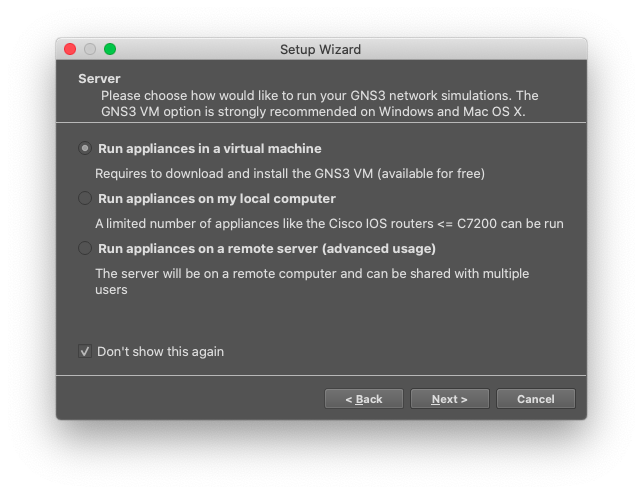
\includegraphics[width=0.8\textwidth]{comparative-gns3-setup-wizard-servers}
  \caption{The GNS3 setup wizard which shows on a fresh installation on by user's demand giving the options running GNS3 distributed}
  \label{fig:comparative-gns3-setup-wizard-servers}
\end{figure}


In GNS3, the project is running in the server, which, in many cases, is not the user's physical computer.
There is a notion of users connecting to the server (the open project), sharing resources and seeing the effects of actions done by action, which may require some protocols of coordination, e.g. given by the instructor.

\subsection{Portability and Sharability of Projects}
\label{subsec:comparativeportability}
In texts offering comparisons between network emulators and simulators~\cite{netkit-full,reproduciblenetexp}---in general, software based solutions to replace ``the real thing''---, this is an aspect that has to be taken into account.

On Kathará, if the default Docker images are used (or, in case they are customized, the extended images are published on Docker Hub, and they can always be) the labs are easily shareable and reproducible with the same behavior.

On GNS3, the aforementioned observation (about Kathará) doesn't hold.
The dependency
  \begin{enumerate*}[label=(\roman*), itemjoin={{, }}, itemjoin*={{, and }}]
  \item on the proprietary images for either Dynamips or IOSv
  \item in case of using IOSv, on a Linux host for QEMU/KVM support
  \item in case of using Docker nodes as end hosts, which the GNS3's computes can only interact with on Linux hosts, on that operating system
  \end{enumerate*}
as well as the possibility to have distributed labs across more than one server, literally separating the whole set of files needed to reproduce an experiment, and the heavy relying on randomly generated UUIDs, make this more difficult by orders of magnitude. % TODO add UUIDs to acronyms

% end of section comparativenonfunctional


% Section "Performance and resource consumption"
\section{Performance and Resource Consumption}
\label{sec:comparativeperformance}

In terms of resource consumption, experiments with GNS3 and Kathará are very different.
That has an impact in the required computer infrastructures and setups required to do the experiments.
As stated in the explanation between containers-as-lightweight-virtual-machines versus standard \glspl{vm}, a container provides a virtual isolation of the filesystem and networking (among others) for its processes while \glspl{vm} need everything, in every layer of software, a regular host has to run (operating system, libraries, applications) to be loaded each time for each running virtual machine.

In a running Kathará or GNS3 topology, there are associated processes to each node.
As previously shown, GNS3's Cisco routers can be \glspl{vm} running the modern Cisco IOSv or processes of the Dynamips emulator which in fact is a virtual machine, but not in the sense of \textquote{a PC running in isolation with virtualized IO} (e.g. the instructions of those IOS images isn't x86, and therefore there has to be a translation to machine instructions).

Table~\ref{tab:comparativeramusage} lists approximate values measured with the \texttt{top} command (and \texttt{docker~stats}, for Kathará's) on more than one GNU/Linux system for the memory consumption of each process that backs a live node in a topology for each studied possibility.
These measures only approximate the order of magnitude, in a sense that can be described as: \textquote{of several different times the values were measured, on more than one machine, they didn't fluctuate more than, say, $50~\mbox{MiB}$ (for GNS3's) or $5~\mbox{MiB}$ (for Kathará's),} and therefore it doesn't correspond to an accurate arithmetic mean or other formal statistical method.

% Table tab:comparativeramusage
\begin{table}
  \centering
  \small
  \begin{tabulary}{0.9\textwidth}{ll}
    \toprule
      \textbf{Topology node}                   & \textbf{Memory usage}\\
    \midrule
      GNS3 -- Cisco IOSvL2 (KVM via QEMU)      & $\approx 460~\mbox{MiB}$\\
      GNS3 -- Cisco c3745 (Dynamips process)   & $\approx 270~\mbox{MiB}$\\
      Kathará (any node is a Docker container) & $\approx 4~\mbox{MiB}$\\
    \bottomrule
  \end{tabulary}
  \caption{%
    Approximate metrics of the memory footprint of (networking) nodes in topologies for different emulators
  }
  \label{tab:comparativeramusage}
\end{table}


For the sake of example, the query for the memory footprint of the running Docker containers on a host (in this case, all of them are Quagga-enabled Linux hosts as Kathará nodes) is shown in figure~\ref{fig:comparative-docker-stats}.

% Figure fig:comparative-docker-stats
\begin{figure}
  \centering
  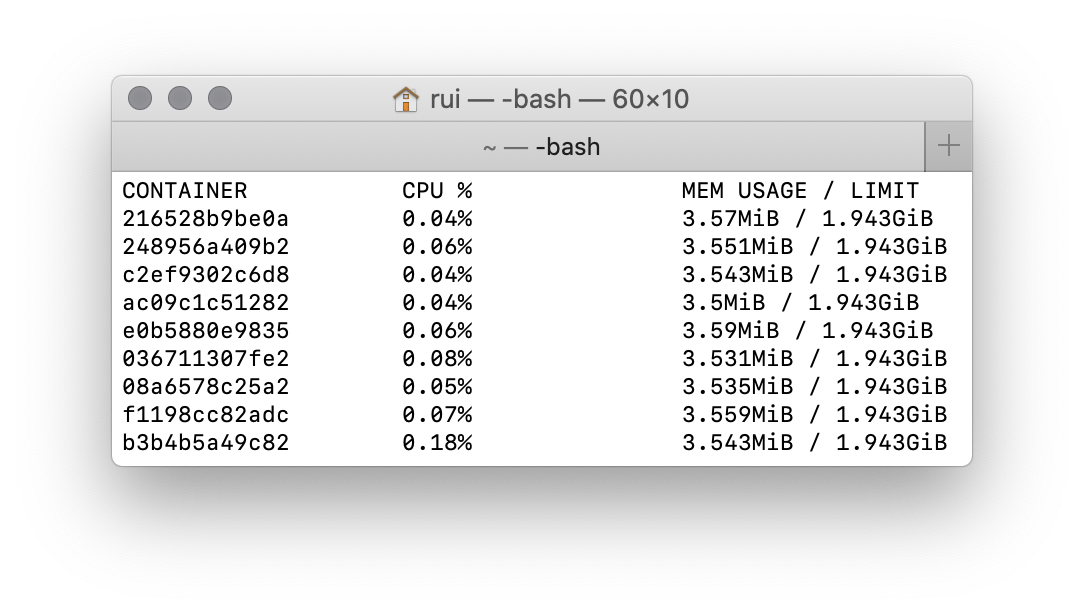
\includegraphics[width=0.8\textwidth]{comparative-docker-stats}
  \caption{The \texttt{docker stats} command showing the resources taken by containers corresponding to nodes in a Kathará lab}
  \label{fig:comparative-docker-stats}
\end{figure}


% end of section comparativeperformance


% end of chapter
